\chapter{Contributions}
\label{ch:contributions}

We concluded previous chapter section \ref{sec:pidforest-conclusion} by mentioning these issues:
\vspace{-0.5em}
\begin{itemize}
    \setlength\itemsep{-0.5em}
    \item Online Anomaly detection
    \item Handling categorical attributes
    \item Concept Drift
\end{itemize}

In this chapter we will present some enhancements that can be made to improve the performance of isolation forest and pidforest.


\section{Feedback guided anomaly detection}
\label{sec:feedback-guided-anomaly-detection}

Anomaly detectors are often used to produce a ranked list of statistical anomalies, which are examined by human analysts in order to extract the actual anomalies of interest. 

This can be exceedingly difficult and time-consuming when most high-ranking anomalies are false positives and not interesting from an application perspective.

Siddiqui et al. \cite{10.1145/3219819.3220083} address this problem and gives a general framework of how we can convert unsupervised anomaly detection to a semi-supervised anomaly detection problem in which a feedback is given by a domain expert which is used to improve the accuracy of the anomaly detection model. 
Feedback guided anomaly discovery can be model in online convex optimization (OCO) framework. 


\subsection{Online convex optimization}
\label{subsec:online-convex-optimization}

OCO is formulated as an iterative game against a potentially adversarial environment where our moves are vectors from a convex set $S$.
At discrete time steps $t$ the game proceeds as follows:

\begin{enumerate}
    \setlength\itemsep{-0.5em}
    \item We select a vector $w_t \in S$.
    \item The environment selects a convex function $f_t:S \rightarrow R$.
    \item We suffer a loss $f_t(w_t)$.
\end{enumerate}

The goal is to select a sequence of vectors with small accumulated loss over time. 
Given, a $T$-step game episode where we play $(w_1, w_2, \dot , w_T)$ against $(f_1, f_2, \dot,f_T)$ the total $T$ step regret is equal to:

\begin{equation}
    \label{eq:regret}
    Regret_T = \sum_{t=1}^{T} f_t(w_t) - \min_{w^* \in S} \sum_{t=1}^{T} f_t(w^*)
\end{equation}

Refer chapter 2 of \cite{10.1561/2200000018} for more details.

\subsection{Modelling in OCO framework}
\label{subsec:query-guided-anomaly-discovery-as-oco}

Query-guided anomaly discovery can also be viewed as a game
where on each round we output an anomaly ranking over the data
instances and we get feedback on the top-ranked instance. We
wish to minimize the number of times we receive "nominal" as the
feedback response.

To put this problem in OCO framework Siqqiqui et al. \cite{10.1145/3219819.3220083} have put some reasonable restrictions on the form of the anomaly detectors that we will consider.
Only family of generalized linear anomaly detectors (GLADs) which are defined by i) a feature function $\phi : D \rightarrow R^n$, which maps data instances to n-dimensional vectors and ii) n-dimensional weight vector $w$ are considered.
In this context anomaly score for an instance $x$ is defined to be $SCORE(x;w) = - \phi \cdot w$ with larger score corresponding to more anomalous instances.


Given, a GLAD parameterization of an anomaly detector, we can now connect query-guided anomaly discovery to OCO\@.

On each feedback round we select a vector $w_t$ for the detector, which specifies an anomaly ranking over instances. 
We receive feedback $y_t$ on the top ranked instance, where $y_t = +1$ if the instance is alien and $y_t = -1$ if it is nominal.

There are three choices of loss function given in the Siddqui et al. \cite{10.1145/3219819.3220083}: i) linear loss ii) log-likelihood loss iii) logistic loss. 

With the experiments, I came to conclusion that overall linear loss performs better than other two in terms of performance, computational complexity, and accuracy.
Hence, throughout this report I will stick only with linear loss.

\begin{defn}
    \label{defn:linear-loss}
    (Linear loss)
    Let $x_t$ be the top-ranked instance in $D$ under the ranking given by $w_t$.
    The linear loss is given by:

    \vspace{-2em}
    \begin{equation}
        \label{eq:linear-loss}
        f_t(w_t) = -y_t SCORE(x_t;w_t) = y_t w_t \cdot \phi (x_t)
    \end{equation}
\end{defn}

Algorithm 1 of Siqqiqui et al. \cite{10.1145/3219819.3220083} gives a general framework in which OCO can be applied on anomaly detector methods for query-guided anomaly discovery.
In the next section we will model the isolation forest and pidforest in OCO framework.


\section{Feedback guided isolation forest}
\label{sec:feedback-guided-iforest}

The isolation forest assigns an anomaly score to an instance $x$ based on its average isolation depth across the randomized forest, ref \ref{alg:PathLength}.
In particular, the score is (a normalized version of) the negative of
this average depth.

We need to define a GLAD model that replicates isolation forest.

\textbf{Define $\phi_e(x)$} be a binary feature that is 1 if instance x goes through the edge and 0 otherwise.
\textbf{Define $w_e$} be the weight of each edge.
\textbf{Define $\phi$}  be a vector that concatenate all the features across the forest in a consistent order.
\textbf{Define $w$}  be a vector that concatenate all the weights across the forest in a consistent order.

Now the modified model for isolation forest is given by the following algorithms:

\vspace{1em}
\begin{algorithm}[H]
    \caption{$feedbackITree(X)$}
    \label{alg:feedback-guided-itree}
    \setstretch{1.2}
    \SetAlgoLined
    \KwComplexity{Time - $O(\psi^2)$, Space - $O(\psi)$}
    \KwInput{$X$ - input data}
    \KwOutput{a $feedbackITree$}

    q $\leftarrow \: RandomChoice(X.attributes)$

    p $\leftarrow \: RandomNumber(X[$splitAttr$].min(), X[$splittAttr$].max())$

    ftree $\leftarrow$ Node \{ left $\leftarrow$ None, right $\leftarrow$ None, 
    
    \qquad\qquad\qquad size $\leftarrow \: X.size$, splitAttr $\leftarrow$ q, 
    
    \qquad\qquad\qquad splitVal $\leftarrow$ p, $w \leftarrow 1$, $\theta \leftarrow 1$\}   \tcp*{$w,\theta$ for mirror descent}

    \If{X.size $>$ 1 and X[splitAttr].numUnique() $>$ 1}{
        $X_{l} \: \leftarrow  \: X.where(q < p)$

        $X_{r} \: \leftarrow  \: X.where(q \geq p)$

        ftree.left $\leftarrow \: feedbackITree(X_{l})$

        ftree.right $\leftarrow \: feedbackITree(X_{r})$
    }

    \Return{ftree}
\end{algorithm}
\vspace{1em}


\vspace{1em}
\begin{algorithm}[H]
    \caption{$unadjustedPathLength(x, T, hlim, e)$}
    \label{alg:unadjustedPathLength}
    \DontPrintSemicolon
    \setstretch{1.2}
    \SetAlgoLined
    \KwComplexity{Time - $O(t\psi)$, Space - $O(1)$}
    \KwInput{$x$ - input instance, $T$ - a $feedbackITree$, $hlim$ - height limit, $e$ - current path length to be initialized to zero when called first time}
    \KwOutput{path length of $x$}

    \If{ (T.right is None) and (T.left is none) and (e $\geq$ hlim)}{

        \Return $e$ \tcp*{removed the adjustment, return unadjusted path length}

    }

    $a \: \leftarrow \: T.splitAttr$

    \tcp{(e + 1) $\rightarrow$ e + (weight of the edge)}

    \If{ $x[a] < T.splitVal$}{
        \Return  $PathLength(x, T.left, hlim, e + T.w)$
    }
    \Else{
        \Return  $PathLength(x, T.right, hlim, e + T.w)$
    }
\end{algorithm}
\pagebreak


\vspace{1em}
\begin{algorithm}[H]
    \caption{$updateWeights(x, T, hlim, \eta, y)$}
    \label{alg:update-weights-iforest}
    \DontPrintSemicolon
    \setstretch{1.2}
    \SetAlgoLined
    \KwComplexity{Time - $O(t\psi)$, Space - $O(1)$}
    \KwInput{$x$ - input instance, $T$ - a $feedbackITree$, $hlim$ - height limit, $\eta$ - learning rate, $y$ - feedback}

    \If{ (T.right is None) and (T.left is none) and (e $\geq$ hlim)}{

        \Return \tcp*{no child node, all weights updated}

    }

    $a \: \leftarrow \: T.splitAttr$

    \If{ $x[a] < T.splitVal$}{

        nextNode $\leftarrow T.left$
        
    }
    \Else{

        nextNode $\leftarrow T.right$
        
    }

    \tcp{mirror descent update}

    $nextNode.\theta \leftarrow nextNode.\theta - \eta * y$

    $nextNode.w \leftarrow nextNode.\theta * (nextNode.\theta \geq 0)$

    $updateWeights(x, \&nextNode, hlim, \eta, y)$
\end{algorithm}
\vspace{2em}

You can find the complete implementation of the  \href{https://github.com/KishoreKaushal/AnomalyDetection/blob/master/isolationforest/FeedbackIsolationForest.py}{feedback guided isolation forest} at this repository: \url{https://github.com/KishoreKaushal/AnomalyDetection}.



\section{Feedback guided PIDForest}
\label{sec:feedback-guided-pidforest}

The anomaly score for PIDForest is the maximum sparsity among all the PIDTrees.
We need to define a GLAD model that replicates pidforest.

\textbf{Define $\phi_{leaf}(x)$} be a binary feature for a $leaf$ node which is 1 if instance $x$ falls in that leaf.
\textbf{Define $w_{leaf}$} be the sparsity of that $leaf$ node.
\textbf{Define $\phi$}  be a vector that concatenate all the features across the forest in a consistent order.
\textbf{Define $w$}  be a vector that concatenate all the weights across the forest in a consistent order.

Now the modified model for pidforest is given by the following algorithms:


\vspace{1em}
\begin{algorithm}[H]
    \caption{$feedbackPIDTree(X, e, start, end, h, k, \epsilon)$}
    \label{alg:feedback-pidtree}
    \DontPrintSemicolon
    \setstretch{1.2}
    \SetAlgoLined
    \KwComplexity{Time - $O(d \psi log(\psi))$}
    \KwInput{$X$ - input data, $e$ - current depth, $[start, \, end]$ - interval for each attribute, $h$ - max depth, $k$ - max partitions, $\epsilon$ - for histogram construction}
    \KwOutput{a $feedbackPIDTree$}

    $ftree$ $\leftarrow$  \{
    
        \qquad \qquad child : EmptyList,
    
        \qquad \qquad depth : e,
    
        \qquad \qquad sparsity : (-1),
        
        \qquad \qquad $w$ : (-1)
        
        \qquad \qquad $\theta$ : (-1)
    
        \qquad \}

        $ftree.cube = Cube(start, end, \& ftree)$

        \tcp{\&x stands for a reference of x}
        $ftree.pointset = Pointset(filter(X, ftree.cube), \& ftree)$ 

        \If{ftree.depth $<$ h and $\vert ftree.pointset \vert > 1$}{ 
            \tcp{if not a leaf node then split}
            
            $ftree.child \leftarrow \: findSplit(...)$

        }
        \Else{
            $ftree.sparsity \leftarrow ftree.cube.logvolume - log(\vert ftree.pointset.X \vert)$
        
            \tcp{$w, \theta$ will be used for mirror descent algorithm}

            $ftree.\theta \leftarrow ftree.w \leftarrow ftree.sparsity$

        }

    \Return{ftree}
\end{algorithm}



\vspace{1em}
\begin{algorithm}[H]
    \caption{$updateWeights(x, T, \eta, y)$}
    \label{alg:update-weights-pidforest}
    \DontPrintSemicolon
    \setstretch{1.2}
    \SetAlgoLined
    \KwComplexity{Time - $O(t\psi)$, Space - $O(1)$}
    \KwInput{$x$ - input instance, $T$ - a $feedbackPIDTree$, $\eta$ - learning rate, $y$ - feedback}

    \If{ $\vert T.child \vert$ == 0}{

        \tcp{mirror descent update}

        $nextNode.\theta \leftarrow nextNode.\theta - \eta * y$

        $nextNode.w \leftarrow nextNode.\theta * (nextNode.\theta \geq 0)$

        \Return{}

    }

    \tcp{get the nextNode where instance $x$ falls}
    
    $updateWeights(x, \&nextNode, hlim, \eta, y)$
\end{algorithm}
\pagebreak

By putting these models in OCO framework our algorithm's accuracy increases. 
Although for a large amount of streaming data the current algorithm is able to handle little-bit of concept drift but as soon the new data diverges too much in value from the data on which these algorithms are trained there are no leaf nodes on which these new instances will fall.
In the next section, I propose a general framework in which this can be handled.

\section{Online anomaly detection}
\label{sec:online-anomaly-detection}


Consider a streaming dataset $D = [x_1, x_2, \dots \dots  ]$ which increases in size as time progresses.
We introduce the timestamp of creation for each tree in the forest.
It can be implemented by having a $timestamp$ field in the tree object.
Then we can get the timestamp of creation for $i^{th}$ tree in the forest by querying $forest[i].timestamp$.
Or, we can use $Dictionary$ data structure indexed by $timestamp$ to implement forest.
Either way is fine and left as implementation detail.

For the discussion let's denote the initial forest as: $F = [T_{t=1}, \dots, T_{t=num\_trees}]$ where $t$ refers to timestamp and let the timestamp be discrete numbers.
Let $W$ be the window size.
Let $D_{t} \subseteq D$ defined as $D_{t} = D[t:t+W] = [x_t, x_{t+1}, \dots, x_{t+W}]$.
Let the model update after each $\delta$ time steps.
The update can be done in following two ways:

\begin{enumerate}
    \item Retrain the model after every $\delta$ time steps by considering the dataset $D_{i * \delta + 1}$ where $i$ is the iteration number.
    \item Discard $\alpha$ fraction of oldest timestamped trees from the forest and create only those many new trees by considering the dataset $D_{i * \delta + 1}$ where $i$ is the iteration number.
    Note that setting $\alpha = 1$ is same as the first way.
\end{enumerate}

Both of the above ways allow us to handle the concept drift. 

\pagebreak


\section{Handling categorical attributes}
\label{sec:handling-categorical-attributes}

Vatsal et al. \cite{NIPS2019_9710} suggested that to handle the categorical dataset we need some inputs from the domain expert to partition the domain set into subsets such that similar elements are grouped together.
For example, given the set of countries we may partition by continents.
Hence, this is similar to a clustering problem.

In this section we will use the Word2Vec (ref \cite{41224}, \cite{NIPS2013_5021}) method from NLP to find the vector embedding of the categorical features.
Here is a brief overview:

\paragraph{Word2Vec} is a two-layer neural net that processes text by vectorizing words.
Its input is a text corpus and its output is a set of vectors: feature vectors that represent words in that corpus.
While Word2vec is not a deep neural network, it turns text into a numerical form that deep neural networks can understand.

\vspace{1em}
\begin{figure}[!ht]
    \label{fig:cat2vec-implementation}
    \centering
    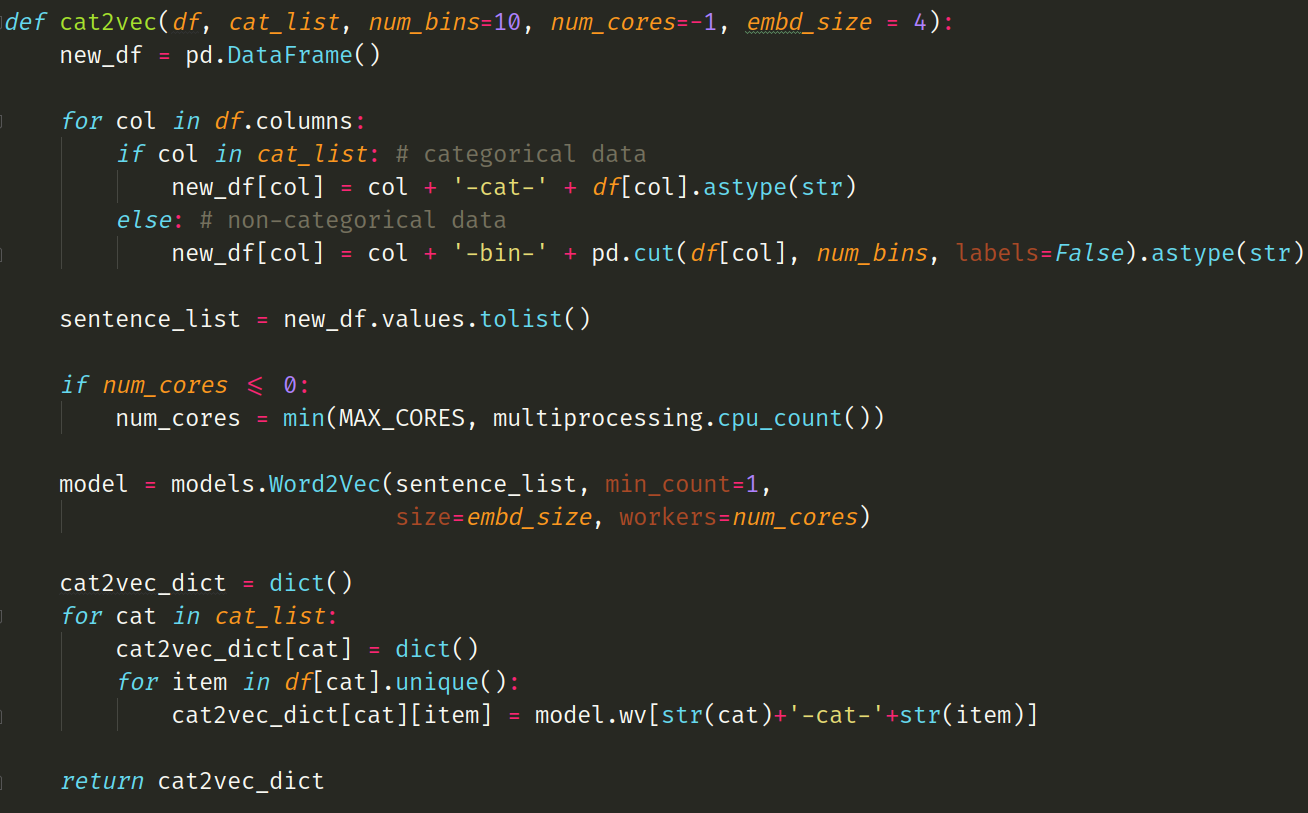
\includegraphics[width=0.9\textwidth]{../fig/chapter4/cat2vec.png}
    \captionsource{cat2vec implementation}
    {\href{https://github.com/KishoreKaushal/AnomalyDetection/blob/master/isolationforest/cat2vec.py}{@KishoreKaushal/AnomalyDetection}}
\end{figure}
\pagebreak

To illustrate, let assume we have 5 APIs running 7 days a week.
Some APIs are used more on weekends while some APIs are used more on weekdays.
We can use cat2vec method to find the similarity measure between API-API, DAY-DAY, and API-DAY.
Here is a sample example:

\vspace{2em}
\begin{figure}[!ht]
    \label{fig:cat2vec-sample-run}
    \centering
    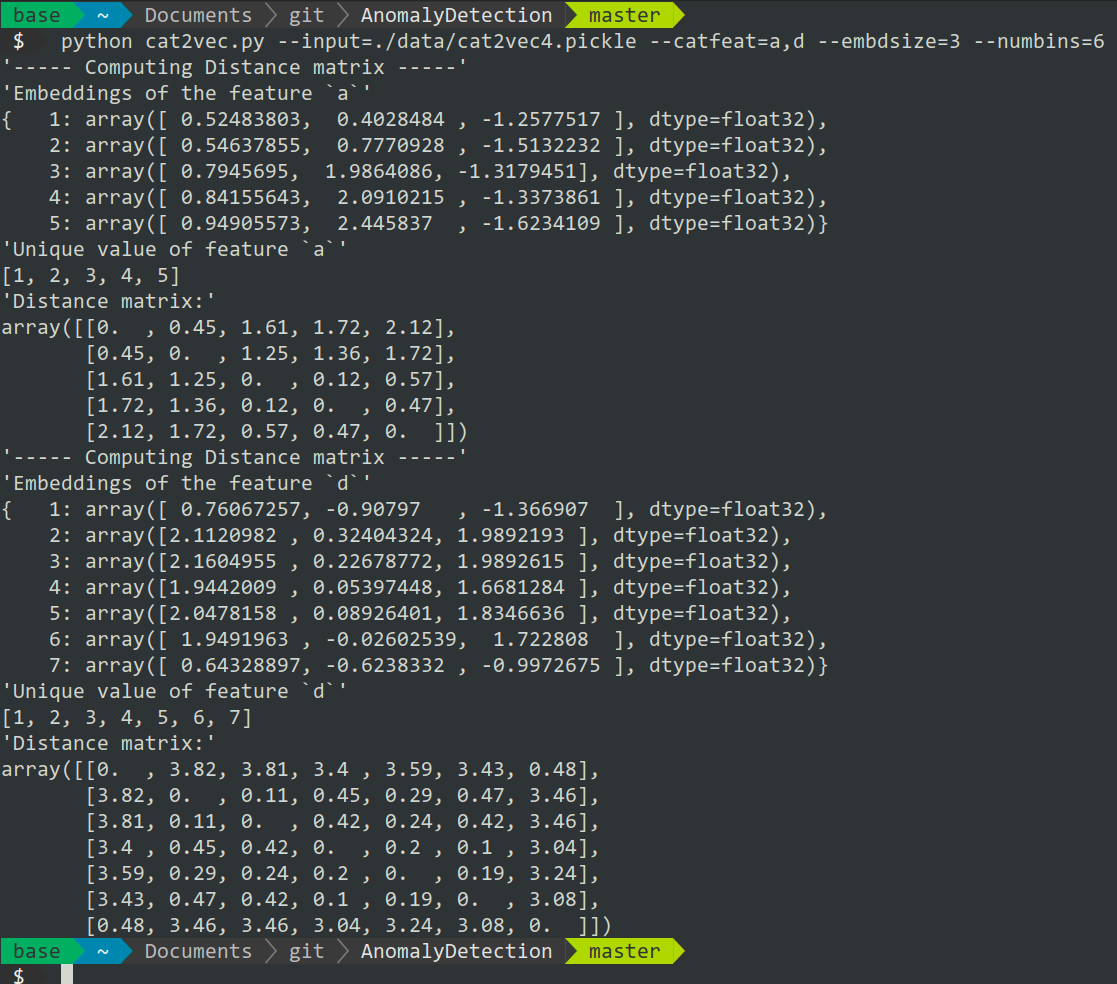
\includegraphics[width=0.9\textwidth]{../fig/chapter4/cat2vec-sample-run.png}
    \captionsource{cat2vec sample run}
    {\href{https://github.com/KishoreKaushal/AnomalyDetection/blob/master/isolationforest/cat2vec.py}{@KishoreKaushal/AnomalyDetection}}
\end{figure}

\begin{figure}[!ht]
    \label{fig:distance-matrix}
    \centering
    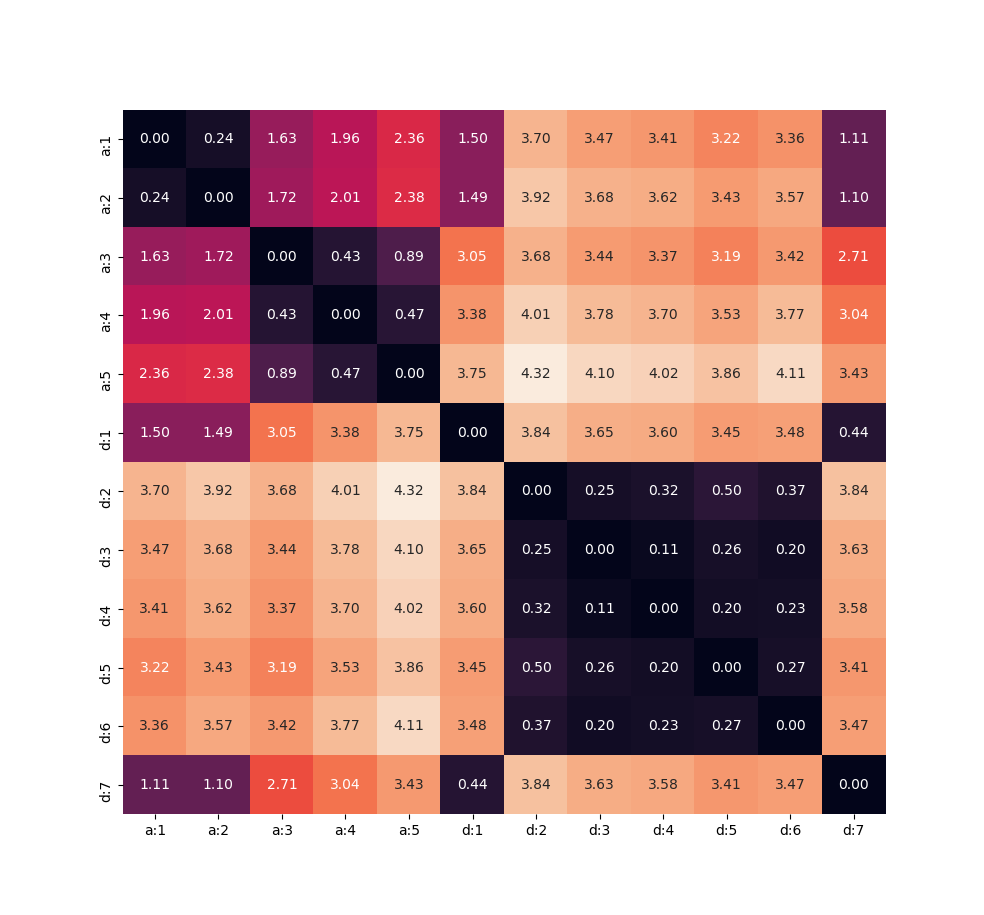
\includegraphics[width=0.7\textwidth]{../fig/chapter4/InterFeatureDistance.png}
    \captionsource{distance matrix}
    {\href{https://github.com/KishoreKaushal/AnomalyDetection/blob/master/isolationforest/cat2vec.py}{@KishoreKaushal/AnomalyDetection}}
\end{figure}



Figure 4.3 is the distance matrix for the sample problem discussed above.
We can use the vector embeddings generated by cat2vec with Isolation Forest and distance matrix for eliminating the need of domain expert to handle the categorical dataset.

\section{Conclusion}
\label{sec:conclusion}

This concludes this report on anomaly detection.
We discussed two state-of-the-art algorithms.
We discussed issues with them and tried to improve upon them on this chapter.
You can find the implementations of these methods and algorithms at my repository.
We are happy to boast that (at present) our code is the only good implementation of PIDForest and feedback guided anomaly discovery available on the internet.

% In the next chapter we will briefly discuss my works on AI in Image Compression, which unfortunately I have to stop in the middle as a consequence of COVID-19 pandemic, because of lack of resources like stable internet and GPU for computation at my home during the lockdown.